\begin{figure}[htbp]
\centering
\begin{tikzpicture}[x=1cm,y=1cm]
\node[anchor=south west,inner sep=0] at (0,0) {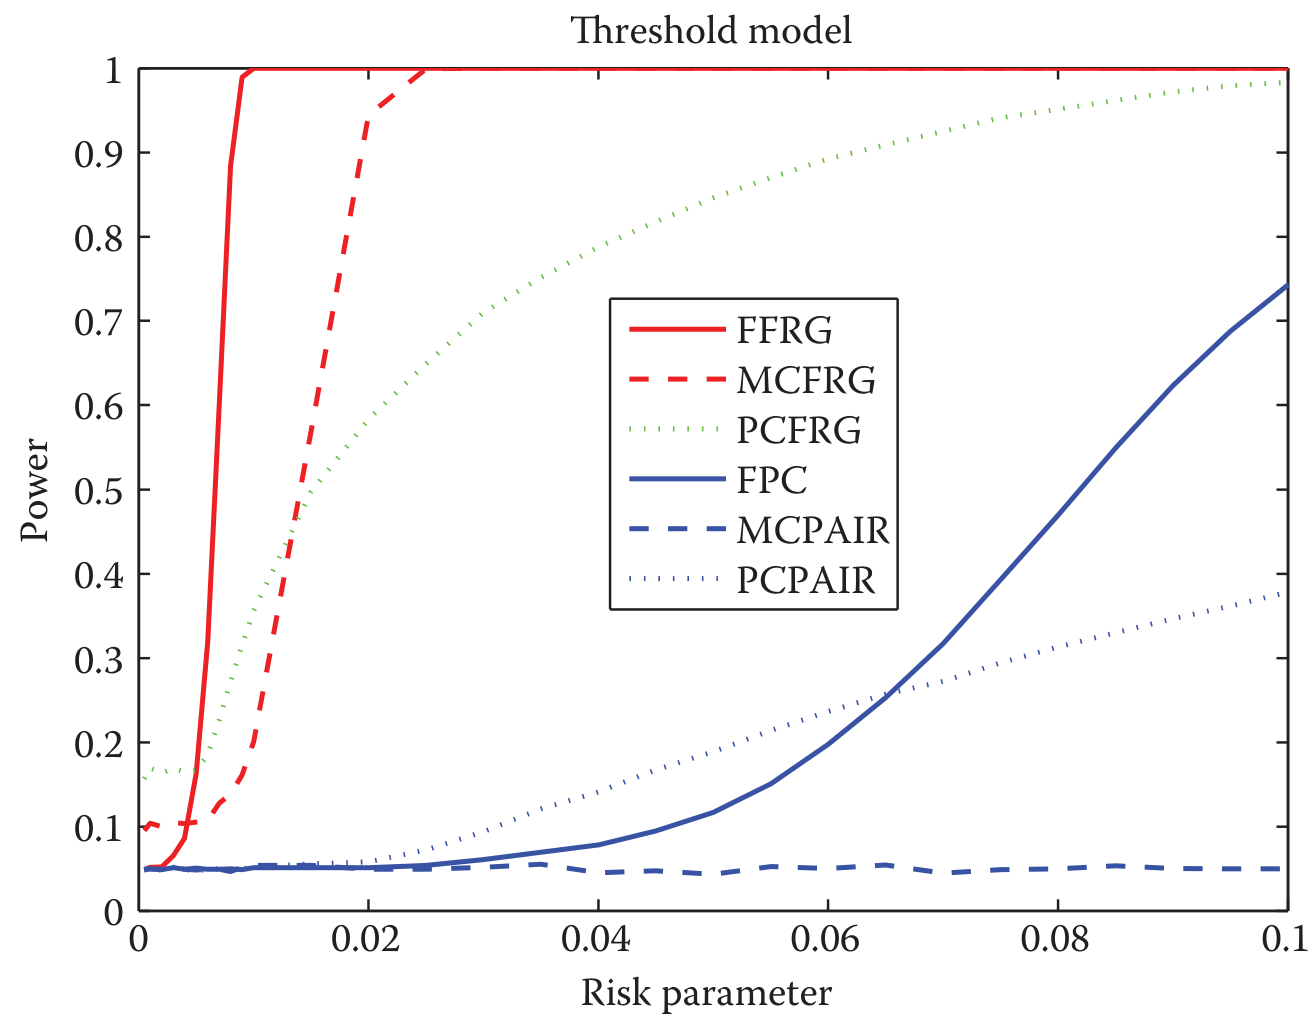
\includegraphics[width=13.8cm]{figures/ch03_fig24_data.png}};
\fill[white] (6.0626,0.0321) rectangle (8.7723,0.5043);
\node[font=\small,rotate=0,inner sep=0] at (7.4174,0.2682) {风险参数};
\fill[white] (0.1494,4.9754) rectangle (0.6321,6.1352);
\node[font=\small,rotate=90,inner sep=0] at (0.3908,5.5553) {统计功效};
\fill[white] (5.9450,10.1204) rectangle (8.9766,10.5927);
\node[font=\small,rotate=0,inner sep=0] at (7.4608,10.3566) {阈值模型};
\end{tikzpicture}
\origfig{24}{阈值模型下六种统计量 F-FRG、MC-FRG、PC-FRG、FPC-FPC、PC-pair-wise 和 MC-pair-wise 的功效曲线。}
\label{fig:ch03-24}
\end{figure}
